\documentclass{beamer}

\usepackage[english]{babel}
\usepackage{amsmath}
\usepackage{amsfonts}
%\usepackage{amsthm}
\usepackage{caption}
\usepackage{bbm}
\usepackage[utf8]{inputenc}
\usepackage[T1]{fontenc}
\usepackage{inconsolata}


\usepackage{tikz-cd}


\usepackage{algorithm}
\usepackage{algpseudocode}
\usepackage{pifont}

\usepackage{color}
\definecolor{bluekeywords}{rgb}{0.13,0.13,1}
\definecolor{greencomments}{rgb}{0,0.5,0}
\definecolor{redstrings}{rgb}{0.9,0,0}

\usepackage{listings}

\lstset{language=[GNU]C++,
showspaces=false,
showtabs=false,
breaklines=true,
showstringspaces=false,
breakatwhitespace=true,
escapeinside={(*@}{@*)},
commentstyle=\color{greencomments},
keywordstyle=\color{bluekeywords}\bfseries,
stringstyle=\color{redstrings},
basicstyle=\ttfamily
}
\newcommand{\bfW}{\mathbf{W}}
\newcommand{\bfw}{\mathbf{w}}
\newcommand{\bfM}{\mathbf{M}}
\newcommand{\bfm}{\mathbf{m}}
\newcommand{\RR}{\mathbb{R}}
\newcommand{\Ss}{\mathcal{S}}
\newcommand{\II}{\mathbb{I}}
\newcommand{\JJ}{\mathbb{J}}
\newcommand{\E}{\mathcal{E}}
\newcommand{\T}{\mathcal{T}}
\newcommand{\VV}{\mathcal{V}}
\newcommand{\MM}{\mathcal{M}}
\newcommand{\NN}{\mathcal{N}}
\newcommand{\e}{\mathbf{e}}
\newcommand{\x}{\mathbf{x}}
\newcommand{\m}{\mathbf{m}}
\newcommand{\h}{\mathbf{h}}
\newcommand{\uu}{\mathbf{u}}
\newcommand{\vv}{\mathbf{v}}
\newcommand{\F}{\mathcal{F}}
\newcommand{\X}{\mathcal{X}}
\newcommand{\CC}{C\nolinebreak\hspace{-.05em}\raisebox{.4ex}{\tiny\bf +}\nolinebreak\hspace{-.10em}\raisebox{.4ex}{\tiny\bf +}}
\def\CC{{C\nolinebreak[4]\hspace{-.05em}\raisebox{.4ex}{\tiny\bf ++}}}
\newcommand{\dP}{\mathcal{P}}
% operator odvoda
\newcommand{\D}{\partial}
%operator 1 + \D
\newcommand{\DD}{\mathcal{D}}
% operator 1+ \D + \D^2 + ...
\newcommand{\sumd}{\tau}
\DeclareMathOperator{\interior}{int}

\DeclareMathOperator{\proj}{pr}

\newtheorem{definicija}{Definicija}[section]
\newtheorem{izrek}{Izrek}[section]
\newtheorem{posledica}{Posledica}[section]
\newtheorem{proposition}{Proposition}[section]
\newtheorem{remark}{Remark}[section]


\usetheme{metropolis} % Use metropolis theme
\title{Operatorski račun nad programskimi prostori}
\date{14. september 2017}
\author{Žiga Sajovic}
\institute{Univerza v Ljubljani, Fakulteta za Računlništvo in Informatiko}
\begin{document}
\maketitle

\begin{frame}{Tematika naloge}
Razvijte algebraični jezik, ki bo deloval kot formalni račun za globoko učenje, hkrati pa bo orodje za proučevanje programov, ki so v njem implementirani. Jezik naj deluje kot poln model globokega učenja. Omogoča naj tako izražanje programov, da bo že njihov zapis nudil teoretični vpogled vanje.
\end{frame}
\section{Reševane pomanjkljivosti}

\begin{frame}{Pomanjkljivosti}
Z delom smo reševali dve družini pomankljivosti:
\begin{itemize}
\item
pomanjkljivosti algebre jezikov
\item
pomanjkljivosti globokega učenja
\end{itemize}
ki ju pred začetkom utemeljimo z mnenji strokovnjakov obeh področij.
\end{frame}

\begin{frame}{Pomanjkljivosti algebre jezikov}

``Von Neumann languages do not have useful properties for reasoning about programs. Axiomatic and denotational semantics are precise tools for describing and understanding conventional programs, but they only talk about them and cannot alter their ungainly properties. Unlike von Neumann languages, the language of ordinary algebra is suitable both for stating its laws and for transforming an equation into its solution, all within the language.''

-- John Backus, \textit{Can Programming Be Liberated From the von Neumann Style?}

\textbf{Posledično nam ne omogoča algebraičnega manipuliranja odvedljivih programov.}

\end{frame}

\begin{frame}{Pomanjkljivosti globokega učenja}
``\dots There is no proper definition of what deep learning even is at this stage. Your [avtorjeva] theory of Operational Calculus on Programming Spaces [naše delo] could offer a first such definition, and a tool for theoretic investigations, through the formalism you [avtor] propose.''

-- dr. Leon Buttou, \textit{v korespondenci z avtorjem}

\textbf{Posledično preiskovanja področja potekajo predvsem empirično.}

\end{frame}

\begin{frame}[fragile]{Komutativen diagram}
\begin{figure}[h]
\begin{center}
\begin{tikzcd}
{} & \parbox{2cm}{\centering \textbf{Programska analiza}}\arrow[dashed]{d}{f}\arrow{ddr}{f_2}\arrow{ddl}{f_1} & {}\\
{} & \textbf{Naše delo}\arrow{dl}{\pi_1} \arrow{dr}{\pi_2} & {}\\
\textbf{Globoko učenje}& {} & \textbf{Formalni jeziki}  
\end{tikzcd}
\end{center}
\end{figure}

Naše delo hkrati rešuje tako pomanjkljivost algebre jezikov kot pomanjkanje formalizma v globokem učenju, in sicer tako, da zgornji diagram komutira.

\end{frame}

\begin{frame}[fragile]{Komutativen diagram}
\begin{figure}[h]
\begin{center}
\begin{tikzcd}
{} & \parbox{2cm}{\centering \textbf{Programska analiza}}\arrow[dashed]{d}{f}\arrow{ddr}{f_2}\arrow{ddl}{f_1} & {}\\
{} & \textbf{Naše delo}\arrow{dl}{\pi_1} \arrow{dr}{\pi_2} & {}\\
\textbf{Globoko učenje}& {} & \textbf{Formalni jeziki}  
\end{tikzcd}
\end{center}
\end{figure}

Tako je na delo mogoče gledati, kot na produkt globokega učenja in formalnih jezikov v kategoriji programske analize.

\end{frame}

\section{Programski prostori}

\begin{frame}{Programski prostor}
Programe bomo modelirali kot preslikave vektorskih prostorov, vase. Če se osredotočimo na realne spremenljivke (tipa float ali double), je trenutno stanje pomnilnika predstavljivo z visoko-dimenzionalnim vektorjem. Množico vseh možnih stanj pomnilnika lahko modeliramo s končno-dimenzionalnim vektorskim prostorom $\VV\simeq\RR^n$ (podobno kot pri \emph{nevronskih Turingovih strojih}).

\textbf{\emph{Programski prostor} je prostor vseh preslikav $\VV\to\VV$, ki se dajo zapisati v obliki programa v izbranem programskem jeziku.}
\end{frame}

\begin{frame}{Evklidski stroj}

\begin{definicija}[Evklidski stroj]
Par $(\VV,\F)$, kjer sta
\begin{itemize}
\item
$\VV$ končno-dimenzionalni vektorski prostor nad obsegom $K$,
\item
$\F<\VV^\VV$ podprostor prostora $\VV^\VV$ vseh preslikav $\VV\to\VV$,
\end{itemize}
imenujemo \emph{Evklidski stroj} (z akcijami iz $\F$ nad $\VV$).
\end{definicija}

\textbf{Na prvi pogled se Evklidski stroj zdi kot opis funkcijskega programiranja s kompozicijami, podedovanimi od $\F$, a ob zajemanju prednosti funkcijskega programiranja ponuja tudi druge prednosti.}
\end{frame}

\section{Odvedljivi programski prostori}

\begin{frame}{Navidezni pomnilniški prostor}

Pomnilniški prostor programa je redko obravnavan kot kaj več kot zgolj shramba. Da pa bi obogatili Evklidski stroj z dodano strukturo, se osredotočimo prav nanj. Ohlapno rečeno je funkcijsko programiranje opisano z monoidi (grupami brez inverzov), zato se (multi)linearno algebraičen opis pomnilnika zdi primeren korak k pridobitvi dodatne strukture.

\textbf{Navidezni pomnilniški prostor je tenzorski produkt pomnilniškega prostora $\VV$ s tenzorsko algebro njegovega duala $T(\VV^*)$.}
\begin{equation*}
\VV_\infty = \VV\otimes T(\VV^*) = \VV\oplus
(\VV\otimes\VV^*)\oplus\ldots\label{eq:virtual-memory}
\end{equation*}

\end{frame}

\begin{frame}{Odvedljiv programski prostor}
\begin{definicija}[Odvedljiv programski prostor]
\emph{Odvedljiv programski prostor} $\dP_0$ je vsak podprostor prostora $\F_0$, kjer
\begin{equation*}\label{eq:P}
 	\D\dP_0\subset\dP_0\otimes T(\VV^*).
\end{equation*}
Prostor $\dP_n<\F_n$, ki ga napenja $\{\D^k\dP_0;\quad 0\le k\le n\}$ nad $K$, imenujemo \emph{odvedljiv programski prostor reda} $n$. Ko so vsi elementi $\dP_0$ analitični, $\dP_0$ imenujemo \emph{analitični programski prostor}. 
\end{definicija}
\end{frame}

\begin{frame}{Odvedljiv programski prostor}
\begin{izrek}[Neskončna odvedljivost]\label{thm:infDif}
Vsak odvedljiv programski prostor $\dP_0$ je \emph{neskončnokrat odvedljiv programski prostor}, kar pomeni,
\begin{equation*}\label{eq:P_n}
	 		\D^k\dP_0\subset\dP_0\otimes T(\VV^*)
	 	\end{equation*}
za vsak $k\in\mathbb{N}$.
\end{izrek}

\begin{posledica}\label{tenProdEmb}
Odvedljiv programski prostor reda $n$, $\dP_n:\VV\to\VV\otimes T(\VV^*)$, lahko vložimo v tenzorski produkt funkcijskega prostora $\dP_0$ in prostora $T_n(\VV^*)$ multi-tenzorjev reda $n$ ali manj:
\begin{equation*}
    \label{eq:D_p_embed}
    \dP_n<\dP_0\otimes T_n(\VV^*).
  \end{equation*}
\end{posledica}

\end{frame}

\begin{frame}{Navidezni tenzorski stroji}

Iz Izreka o Neskončni odvedljivosti in njegovi Posledici sledi, da par $(\VV, \dP_0)$ -- skupaj s strukturo tenzorske algebre $T(\VV^*)$ -- zadošča za konstrukcijo odvedljivih programskih prostorov $\dP_\infty$ z uporabo linearne kombinacije elementov $\dP_0\otimes T(\VV^*)$. 

\textbf{Zato par $(\VV, \dP_0)$ s pripadajočim navideznim pomnilniškim prostorom $\VV\otimes \T(\VV^*)$ poimenujemo navidezni tenzorski stroj, v katerem so osnovni programi tenzorski mreže}
\begin{equation*} \label{eq:tenWord}
\NN(v)=\phi_k\circ W_k\circ\cdots\circ\phi_0\circ W_0(v).
\end{equation*}

\end{frame}

\section{Operatorski račun nad programskimi prostori}

\begin{frame}{Razvoj v tenzorsko vrsto}
Naslednje, kar naš model potrebuje, je operator, ki bi prestavil vrednost
funkcije iz njene začetne vrednosti. \textbf{Tak operator bi lahko kasneje uporabili
za implementacijo iteratorjev in komponerjev.}
\end{frame}

\begin{frame}{Razvoj v tenzorsko vrsto}
Takšen operator definiramo kot
\begin{equation*}
 	e^{h\D}=\sum\limits_{n=0}^{\infty}\frac{(h\D)^n}{n!}
 \end{equation*}
 Torej je operator $e^{h\D}$ preslikava med programskimi prostori
  \begin{equation*}
  	e^{h\D}:\dP\to\dP_\infty.
  \end{equation*}
 \textbf{Hkrati pa definira preslikavo}
   \begin{equation*}\label{eq:specProg}
   	e^{h\D}:\dP\times \VV\to \VV\otimes \T(\VV^*),
   \end{equation*}
\textbf{iz prostora programov v prostor multi-linearnih preslikav.}
\end{frame}

\begin{frame}{Razvoj v tenzorsko vrsto}

\begin{izrek}[Razvoj v tenzorsko vrsto]\label{izr:e^d}
	Za program $P\in\dP$  se razvoj v neskončno tenzorsko vrsto
  v točki $\vv_0\in \VV$ izraža z več kontrakcijami 
	\begin{multline*}\label{eq:tenzorVrsta}
	P(\vv_0+h\vv) = \Big((e^{h\D}P)(\vv_0)\Big)(\vv)
  = \sum_{n=0}^\infty\frac{h^n}{n!}\D^nP(\vv_0)\cdot (\vv^{\otimes n})\\
  = \sum_{n=0}^\infty \frac{h^n}{n!}\sum_{\forall_{i,\alpha}}\frac{\partial^nP_i}{\partial
 		    x_{\alpha_1}\ldots \partial x_{\alpha_n}}\e_i\cdot
 		  dx_{\alpha_1}(\vv)\cdot\ldots \cdot dx_{\alpha_n}(\vv).
	\end{multline*}
\end{izrek}

\end{frame}

\begin{frame}{Uporaba}
Predstavljena teorija ponuja več zmožnosti: 
\begin{itemize}
\item
algebraične manipulacije programov
\item
uporaba operatorjev kot oblika abstrakcije
\item
izpeljave teoretično utemeljenih modelov globokega učenja
\item
poenotenje teorije avtomatskega odvajanja
\item
funkcijske transformacije in prevedbe programov
\item
itd.
\end{itemize}
\end{frame}

\section{Implementacija}
\begin{frame}{GitHub}
\begin{figure}[h]
\centering
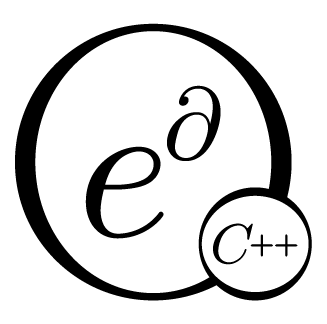
\includegraphics[width=0.5\linewidth]{edCpplogo.png}
\end{figure}
Odprtokodna implementacija odvedljive različice jezika $\CC$ je dostopna na avtorjevi GitHub strani.
\end{frame}
\end{document}